\documentclass[portrait,a0paper]{baposter}

\usepackage{calc}
\usepackage{url}
\usepackage{amsmath}
\usepackage{amssymb}
\usepackage{relsize}
\usepackage{multirow}
\usepackage{booktabs}
\usepackage{graphicx}
\usepackage{multicol}
\usepackage[T1]{fontenc}
\usepackage{ae}
\usepackage{mathrsfs}
\usepackage{ifpdf}
\usepackage{wallpaper}

\renewcommand{\familydefault}{\sfdefault}

\ifpdf
	\pdfcompresslevel=9
	\pdfinfo
	{
		/Author (Luis Sanabria-Russo, Jaume Barcel\'{o}, Boris Bellalta)
		/Title (Fairness in Collision-Free WLANs)
		/Subject (Poster for INFOCOM 2013)
	}
\fi

\selectcolormodel{cmyk}

\definecolor{imdeanavy}{cmyk}{1,0.342,0,0.714}
%\definecolor{imdeabluedark}{cmyk}{0.628,0.345,0,0.431}
\definecolor{imdeabluedark}{cmyk}{0.23,0.11,0,0.33}
\definecolor{imdeabluelight}{cmyk}{0.372,0.208,0,0.114}
\definecolor{imdeacyan}{cmyk}{0.091,0.050,0,0.055}

\newenvironment{packeditemize}{
\begin{itemize}
	\setlength{\itemsep}{1pt}
	\setlength{\parskip}{0pt}
	\setlength{\parsep}{0pt}
}{\end{itemize}}

\begin{document}

\background
{
\begin{tikzpicture}[remember picture,overlay]%
\draw (current page.north west)+(-3.9pt,3.5pt) node[anchor=north west]
{
		\ifpdf
			
\includegraphics[width=\paperwidth+0.7pt]{background2-eps-converted-to.pdf}\\
		\else
			
\includegraphics[width=\paperwidth+0.7pt]{background2.eps}\\
		\fi
};
\end{tikzpicture}%
}

\begin{poster}
% Settings
{
	grid=no,
	columns=2,
	colspacing=1em,
	eyecatcher=no,
	borderColor=imdeanavy,
	textborder=rectangle,
  	titleColor=white,
    	authorColor=white,
	headerfont=\textsf,
	headerborder=closed,
	headershape=rectangle,
	headerColorOne=imdeabluedark,
	headerColorTwo=imdeabluedark,
	headerFontColor=white,
	boxColorOne=white,
	boxColorTwo=imdeacyan,
	boxshade=shade-tb,
	background=user,
	bgColorOne=imdeacyan,
	bgColorTwo=imdeabluelight,
	headerheight=0.12\textheight,
	linewidth=1pt
}
% Eye Catcher
{
}
% Title
{Fairness in Collision-Free WLANs\\ 
\normalsize INFOCOM 2013, Turin, Italy}
% Authors
{
	Luis Sanabria-Russo, Jaume Barcel{\'o}, Boris Bellalta
	%\vspace{0.5em}
	\\
	\normalsize Universitat Pompeu Fabra, Barcelona, Spain
}


% Logo
% {
% \begin{minipage}{17em}
% 	\begin{center}
% 		\ifpdf
% 			
\includegraphics[width=15em]{NeTS-logo-eps-converted-to.pdf}\\
% 		\else
% 			
\includegraphics[width=15em]{NeTS-logo.eps}\\
% 		\fi
% 	\end{center}
% \end{minipage}
% }

\headerbox{Motivation}{name=motivation,column=0,row=0,span=2}
{

Wireless networks are composed of nodes that must contend for the medium in a distributed manner. If two or more contenders attempt transmission at the same time, a collision occurs. %Collisions are intelligible for the receiver, forcing colliding nodes to restart the contention for the medium.

Collisions are the main cause of throughput degradation in wireless local area networks (WLANs), so by constructing collision-free WLANs one can attain greater levels of throughput.

% \begin{itemize}
%  \item What is a contention protocol for?: explain that the medium is shared.
%  \item Highlight that it is widely used by current WiFi devices.
%  \item What are the repercussions of a collision?
% \end{itemize}

}

\headerbox{CSMA/CA}{name=contention,column=0,below=motivation}{

Carrier Sense Multiple Access with Collision Avoidance (CSMA/CA) is the most widely used protocol for medium access control (MAC) in WLANs. CSMA/CA's job is to coordinate access to the medium for each contender.
\\\\
%Time in WLANs is slotted, so CSMA/CA divides it into empty, collision and successful transmission time slots. 
%\\\\
When a node has something to transmit:
\begin{itemize}
	\item Picks a random backoff counter $B\in[0,CW(k)-1]$, where $CW(k)=2^{k}CW_{\min}$ is the contention window, with $CW_{\min}$ its minimum value.
	\item Each passing empty slot decrements $B$ by one. Contenders attempt transmission when the counter expires ($B=0$).
	\item If there is a collision:
	\begin{itemize}
		\item Colliding nodes increment the backoff stage ($k$) in one.
	\end{itemize}
	\item After a successful transmission, the contender resets is backoff stage ($k=0$).
\end{itemize}

%It might be appropriate to detail the behavior of CSMA/CA and CSMA/ECA. A balls and bins figure?

\begin{center}
\begin{tikzpicture}
\path
	\ifpdf
		(0,0) node{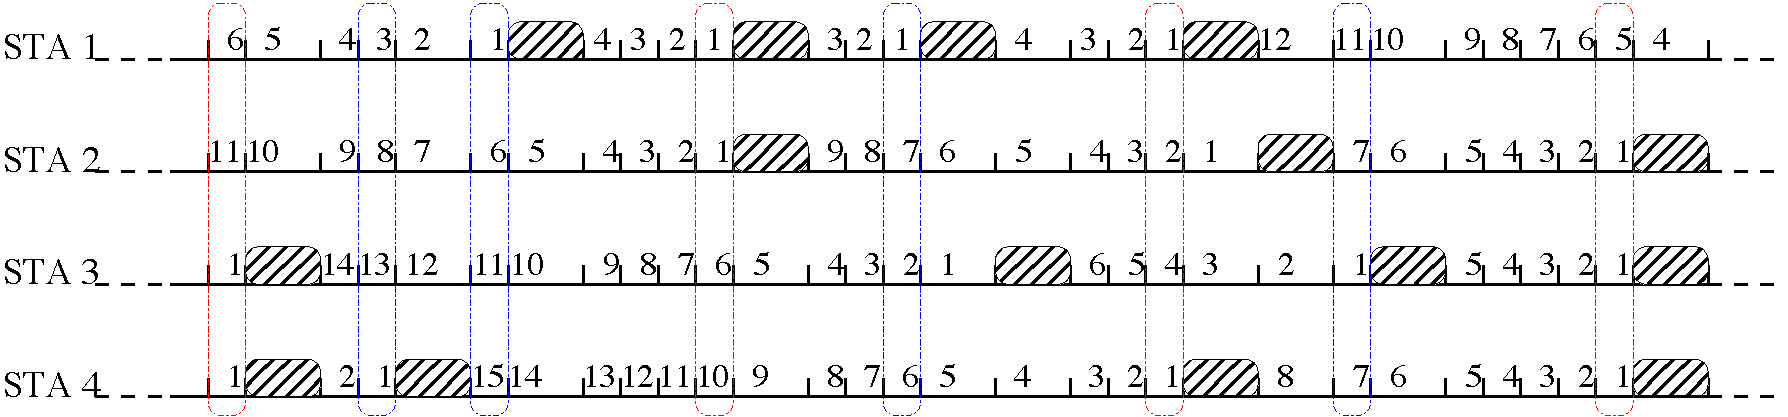
\includegraphics[width=\linewidth]{csma_ca_short.pdf}}
	\else
		(0,0) node{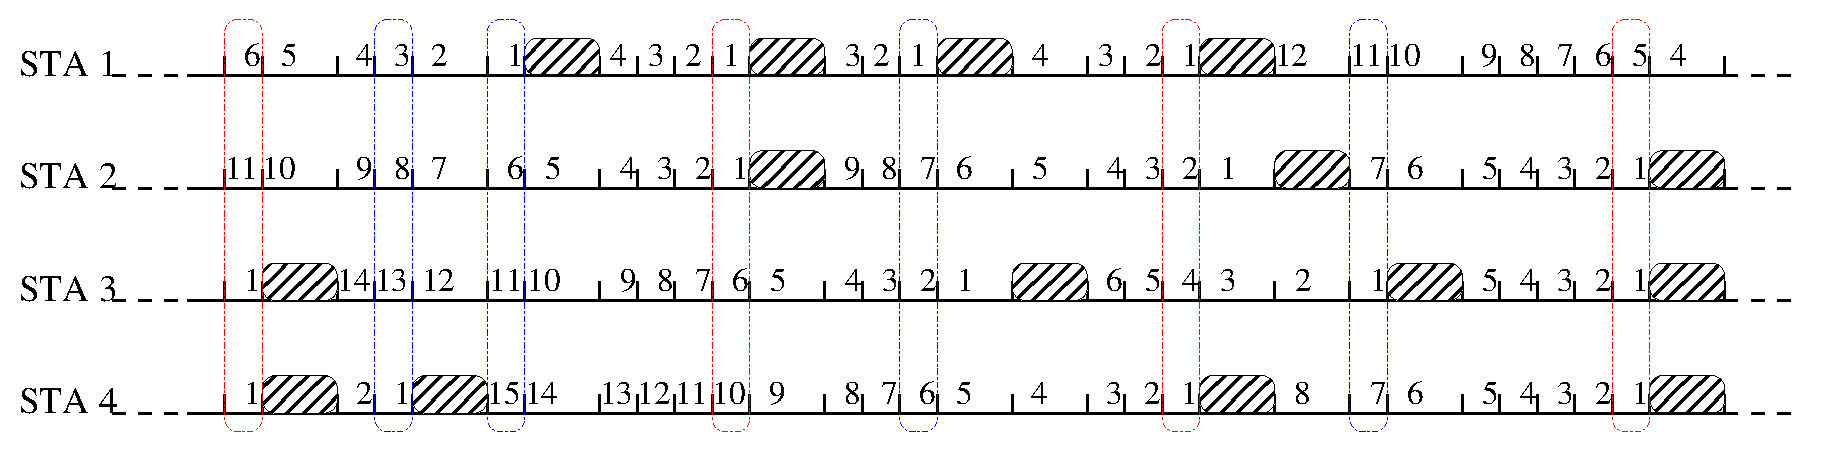
\includegraphics[width=\linewidth]{csma_ca_short.eps}}
	\fi
	(0,-1.7) node {\smaller Example CSMA/CA behavior ($CW_{\min}=16$).};
\end{tikzpicture}
\end{center}
}

\headerbox{Basic ECA}{name=hysteresis,column=0,below=contention}{

CSMA/CA relies in a random backoff counter ($B$) which by its nature generates collisions. Furthermore, CSMA/CA instructs nodes to reset the backoff stage ($k$) after a successful transmission: increasing the collision probability. 
\\\\
Carrier Sense Multiple Access with Enhanced Collision Avoidance~\cite{CSMA_ECA} (Basic CSMA/ECA): 
\begin{itemize}
	\item Picks a deterministic backoff counter $B_{d}=CW_{\min}/2$ after successful transmissions.
	\item Achieves a collision-free state.
	\item Basic CSMA/ECA's throughput goes beyond CSMA/CA's.
\end{itemize}

\begin{center}
\begin{tikzpicture}
\path
	\ifpdf
		(0,0) node{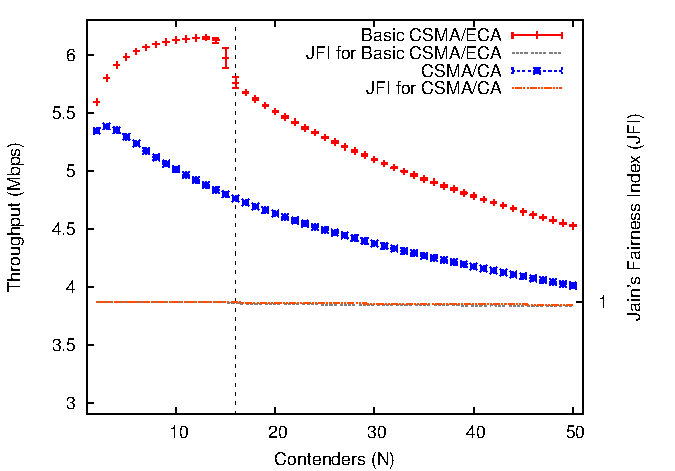
\includegraphics[width=0.7\linewidth]{ECA-vs-CA-FINAL-eps-converted-to.pdf}}
	\else
		(0,0) node{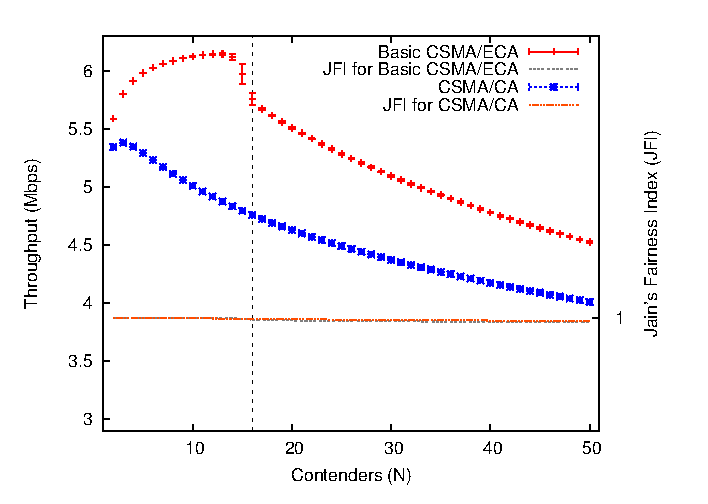
\includegraphics[width=0.7\linewidth]{ECA-vs-CA-FINAL.eps}}
	\fi
	(0,-3.15) node {\smaller Throughput and fairness in CSMA/CA and Basic CSMA/ECA ($CW_{\min}=32$).};
\end{tikzpicture}
\end{center}

Nevertheless, when the number of contenders surpasses $CW_{\min}/2$, the system incurs in a mixed behavior; some nodes pick a random and others a deterministic backoff counter. This setup has undesired repercussions in the attained throughput, approximating Basic CSMA/ECA's to CSMA/CA's.

}

% \headerbox{Throughput and fairness in CSMA/CA and CSMA/ECA}{name=throughputBasicECA,column=0,below=hysteresis,above=bottom}{
% 
% Explaining why the throughput figures look as they do.
% 
% Also it is worth to mention the fair nature of both protocols.
% \begin{center}
% \begin{tikzpicture}
% \path
% 	\ifpdf
% 		(0,0) node{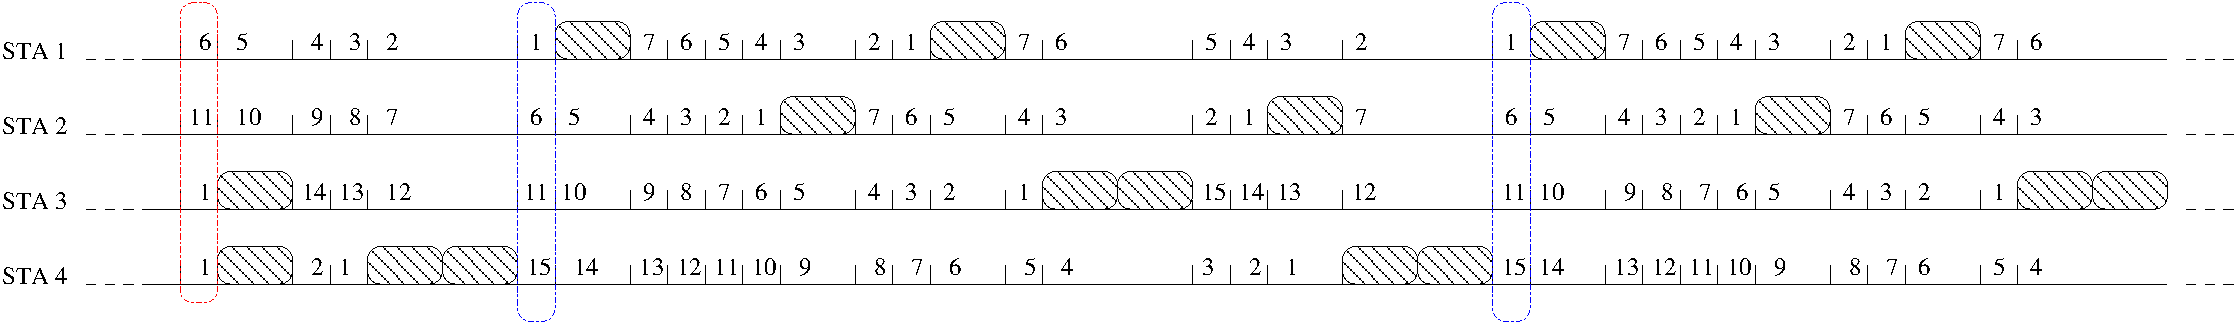
\includegraphics[width=\linewidth]{csma_eca_different_backoff-eps-converted-to.pdf}}
% 	\else
% 		(0,0) node{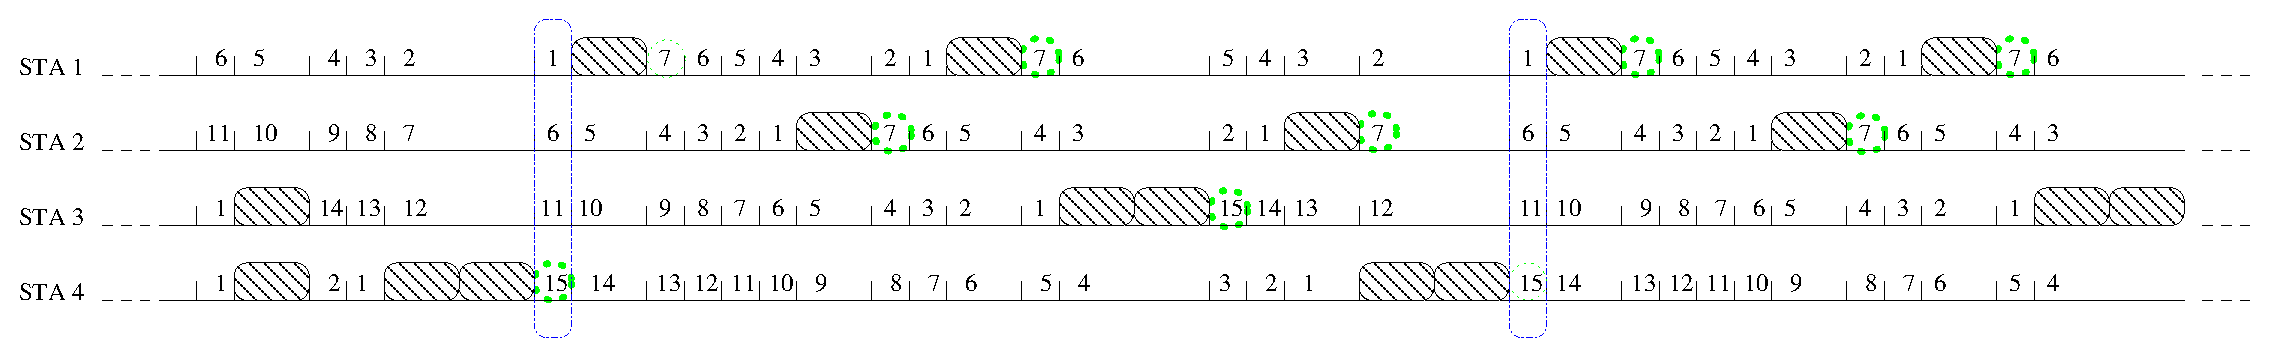
\includegraphics[width=\linewidth]{csma_eca_different_backoff.eps}}
% 	\fi
% 	(0,-1.0) node {\smaller Example CSMA/ECA behavior.};
% \end{tikzpicture}
% \end{center}
% 
% }

\headerbox{CSMA/ECA + hysteresis and fair share}{name=fullECA,column=1,span=1,below=motivation}{

CSMA/ECA is totally distributed, that means that the number of nodes is unknown to all contenders. So, to make it possible to achieve a collision-free state with more than $CW{\min}/2$ contenders, CSMA/ECA:
\begin{itemize}
	\item Instructs nodes {\bfseries not} to reset their backoff stage after successful transmissions.
	\item Picks a new deterministic backoff $B_{d}=CW(k)/2$.
\end{itemize}
We called this measure \emph{hysteresis}.
\\\\
With hysteresis some nodes may have larger $B_{d}$ than others. This unfairness issue is averted by:

\begin{itemize}
	\item Allowing nodes at backoff stage $k$ to send $2^{k}$ packets. 
\end{itemize} 

This is called \emph{fair share}~\cite{fairness-ECA}.

\begin{center}
\begin{tikzpicture}
\path
	\ifpdf
		(0,0) node{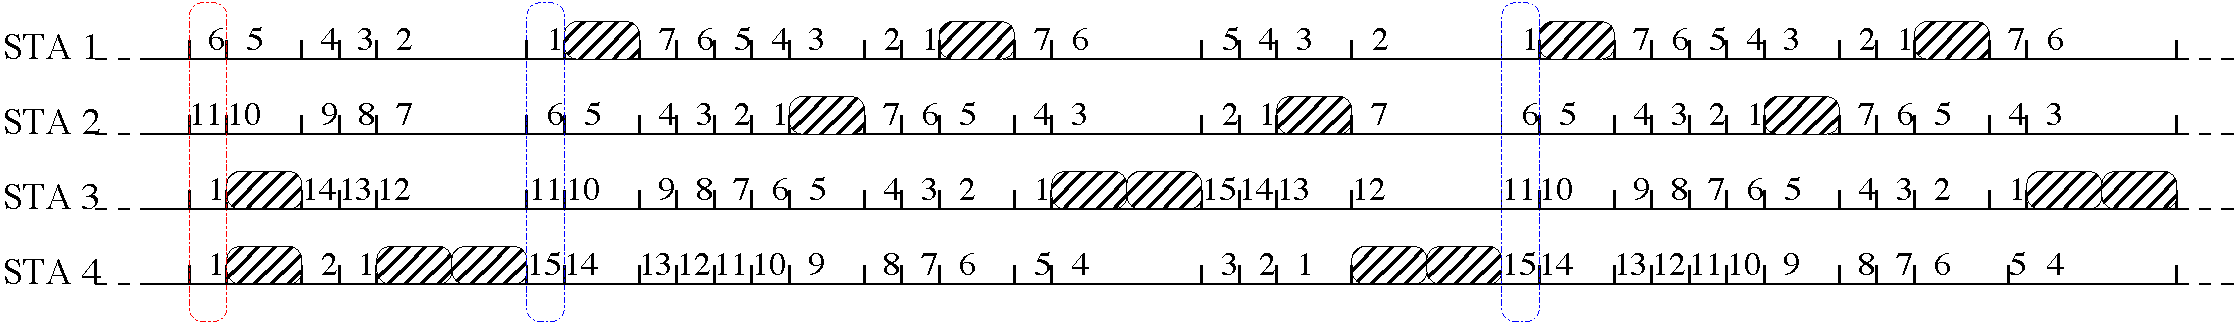
\includegraphics[width=\linewidth]{csma_eca_different_backoff_short.pdf}}
	\else
		(0,0) node{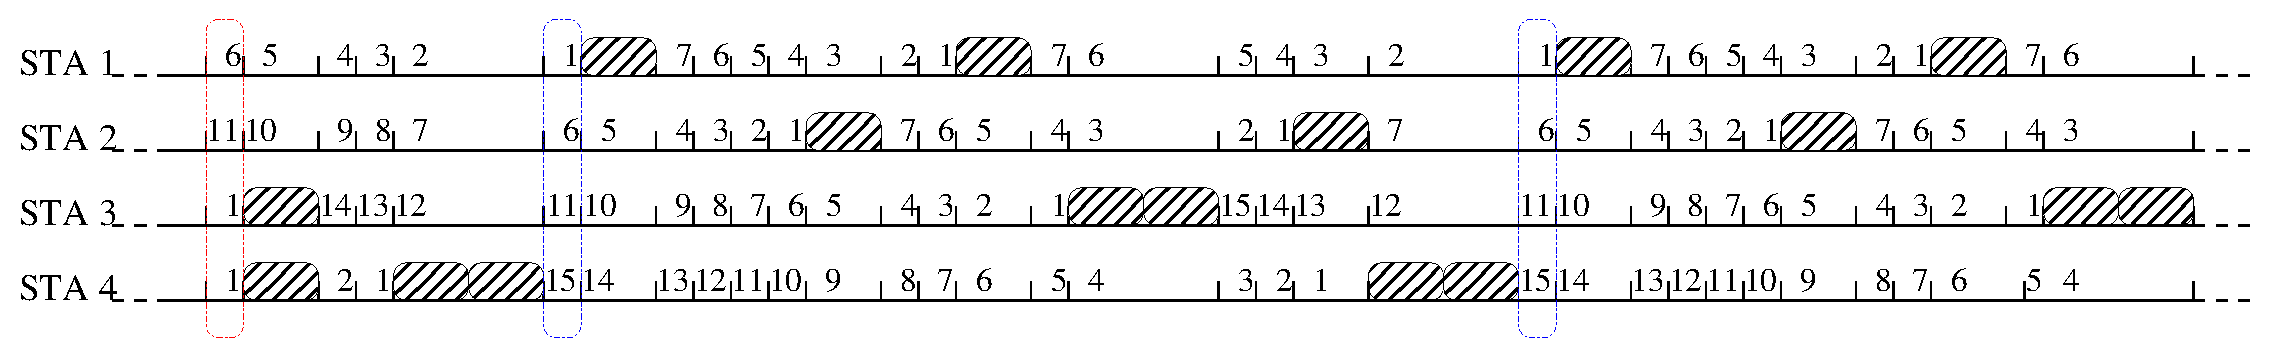
\includegraphics[width=\linewidth]{csma_eca_different_backoff_short.eps}}
	\fi
	(0,-1.3) node {\smaller Example CSMA/ECA behavior with hysteresis and fair share ($CW_{\min}=16$).};
\end{tikzpicture}
\end{center}

\begin{center}
\begin{tikzpicture}
\path
	\ifpdf
		(0,0) node{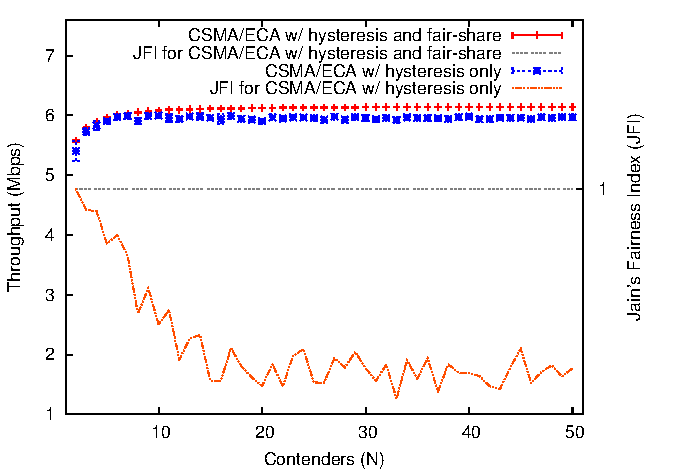
\includegraphics[width=0.7\linewidth]{ECA-w-enhancements-FINAL-eps-converted-to.pdf}}
	\else
		(0,0) node{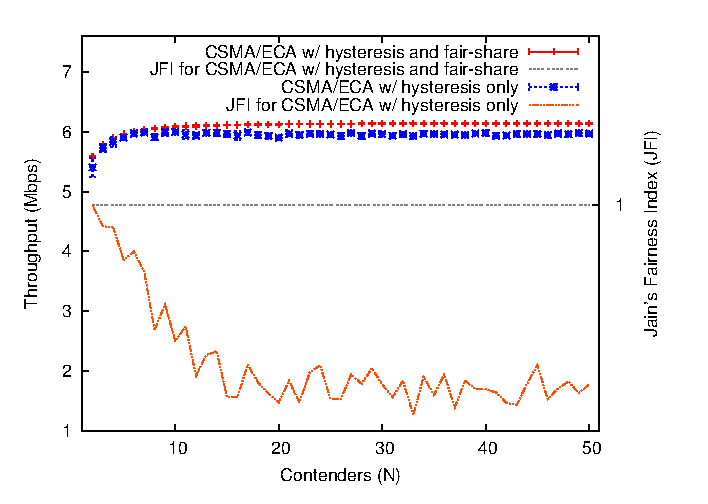
\includegraphics[width=0.7\linewidth]{ECA-w-enhancements-FINAL.eps}}
	\fi
	(0,-3) node {\smaller Throughput and fairness when incorporating hysteresis and fair share to CSMA/ECA.};
\end{tikzpicture}
\end{center}

}

\headerbox{Conclusions and Future plans}{name=future,column=1,below=fullECA}{

Hysteresis allows CSMA/ECA to allocate any number of contenders in a collision-free state, while fair share compensates the unfairness issue; allowing CSMA/ECA to attain greater throughput than CSMA/CA under most typical conditions.
\\\\
As future work, we plan to:
\begin{itemize}
	\item Test CSMA/ECA under non-saturated scenarios.
	\item Implement IEEE 802.11e EDCA quality of service measures.
	\item Implement CSMA/ECA in cheap commodity hardware~\cite{WMP}.
\end{itemize}
}

\headerbox{References}{name=references,span=1,column=1,above=bottom}{

{
 \scriptsize
 
 \renewcommand*{\refname}{\vspace*{-0.5em}}
 \let\oldbibliography\thebibliography
 \renewcommand{\thebibliography}[1]{\oldbibliography{#1}\setlength{\itemsep}{-0.3em}}

% \bibliographystyle{Classes/IEEEtran}
% \bibliography{IEEEabrv,ref}

 \begin{thebibliography}{1}
% 
 \bibitem{CSMA_ECA}
Barcelo, J. and Toledo, A.L. and Cano, C. and Oliver, M.
\newblock Fairness and Convergence of CSMA with Enhanced Collision Avoidance (ECA).
\newblock {\em 2010 IEEE International Conference on Communications (ICC)} , may 2010, pp 1--6.

 \bibitem{fairness-ECA}
Sanabria-Russo, L. and Barcelo, J. and Bellalta, B.
\newblock Fairness in Collision-Free WLANs.
\newblock {\em ArXiv e-prints} , February 2013.

 \bibitem{WMP}
Tinnirello, I. and Bianchi, G. and Gallo, P. and Garlisi, D. and Giuliano, F. and Gringoli, F.
\newblock Wireless MAC processors: Programming MAC protocols on commodity Hardware.
\newblock {\em INFOCOM, 2012 Proceedings IEEE} , march 2012, pp 1269--1277.

\end{thebibliography}
}

}

\end{poster}

\end{document}
